
\chapter{Estado del Arte}
\label{cha:Estado del Arte}

\section{Marco de Referencia Teórico} % (fold)
\label{sec:Marco de Referencia Teórico}

\subsection{Conceptos Generales de una SD-WAN}
\label{sec:Conceptos Generales de una SD-WAN}
SD-WAN  \textbf{(“Software Defined Networking in Wide Area Networks”)} es una aplicación específica de la tecnología de redes SDN \textbf{("en inglés Software Defined Networking, SDN")} aplicada a las conexiones WAN  \textbf{("Wide Area Network en inglés")} utilizadas para conectar redes empresariales sobre grandes distancias geográficas suministrando una arquitectura "Overlay" moviendo el plano de control a la nube, sea esta pública o privada. Según SDN  \textbf{("en inglés Software Defined Networking, SDN")} central, puede definirse como un enfoque de software centrico a las tecnologías de "Networking" que reducen los costos operacionales y de capital ("Capex y Opex") mediante un control programático de la infraestructura de red, facilitando la optimización e innovación.
\\
\subsection{Modelos de Programabilidad de Red}
\label{sec:Modelos de Programabilidad de Red}

Existen actualmente 4 modelos de programabilidad de red, considerados como arquitecturas SDN  \textbf{("en inglés Software Defined Networking, SDN")}, la diferenciación fundamental entre los 4 modelos consiste en la forma como el plano de control se comunica con el plano de datos de los dispositivos, estos modelos pueden resumirse como sigue:
\begin{itemize}
\item[•] \textbf{APIs programables:}  la primera aproximación a SDN  \textbf{("en inglés Software Defined Networking, SDN")} es la inclusión de API \textbf{(del inglés API: Application Programming Interface)} dentro de los dispositivos de red, en este modelo sin embargo no hay un desacoplamiento de los planos de datos y control y estos siguen estando dentro, los equipos de red se comunican directamente con las aplicaciones a través de APIs \textbf{(del inglés API: Application Programming Interface)} u otro mecanismo como NETCONF \textbf{El Protocolo de Configuración de Red}. \textbf{Ver figura 4.1(a) Apis Programables}.

\item[•] \textbf{SDN Clásico}: En este modelo el plano de control y el plano de datos si se encuentran desacoplados completamente, el plano de control se comunica con las aplicaciones mediante APIs \textbf{(del inglés API: Application Programming Interface)} y con el plano de datos mediante \textit{"Openflow"} u otro protocolo propietario. \textbf{Ver figura 5.1(b) SDN Clásico}.

\item[•] \textbf{SDN Híbrido:} funciona bajo el mismo concepto que la arquitectura clásica de SDN  \textbf{("en inglés Software Defined Networking, SDN")}, con la diferencia de que en este caso los dispositivos mantienen su propio plano de control pero siguen comunicándose con las aplicaciones a través de \textit{"Openflow"} mediante una controladora que mantiene el plano de control de todos los equipos. \textbf{Ver figura 5.1(c) SDN Híbrido}.

\item[•]\textbf{Virtualización de Red:} la tendencia de la virtualización ha dividido las redes en un dominio físico y uno virtual, la tendencia es que las decisiones de enrutamiento y seguridad se hagan por software en el plano de virtualización, la comunicación entre este plano virtual y el físico se realiza mediante tecnologías desarrolladas por los fabricantes de software de virtualización, uno de los ejemplos más conocidos es NFX \textbf{"(en inglés: Neutral czFree eXchange)"}. \textbf{Ver figura 5.1(d) Virtualización de Red}.

\begin{figure}[htbp]
 \ref{fig:sdxcentral} \textbf{Tomado de:} \textit{sdxcentral.com Modelos  Programables}.
  \centering
  %\subcaptionbox{\label{fig:leftsubfig}}%
    {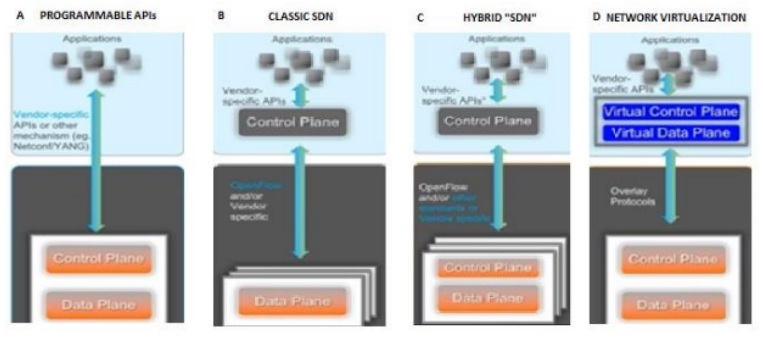
\includegraphics[width=0.7\linewidth]{figure11}}%
%  \subcaptionbox{Another sub-figure\label{fig:rightsubfig}}%
%    {
\includegraphics[width=0.5\linewidth]{knitting-vectorial}}%
  \caption{Modelos Programables de Red}
  \label{fig:sdxcentral}
\end{figure}

\end{itemize}
\subsection{Network Function Virtualization (NFV)}
%\label{sec:Network Function Virtualization (NFV)}

\textit{Network Function Virtualization o NFV ofrece una nueva forma de diseñar, aprovisionar y administrar los servicios de red, desacoplando las funciones de los hardware propietarios y realizando funciones en software como NAT \textbf{(del inglés "Network Address Translation")}, firewall y DNS \textbf{Domain Name System o Sistema de Nombres de Dominio} por nombrar algunos ejemplos. Esta tecnología se encuentra diseñada para consolidar los componentes de red requeridos para lograr una \texttt{infraestructura completamente$\{$virtualizada$\}$} \footnote{http://www.5gamericas.org/es/newsroom/press-releases/nfv-controlando-las-redes-virtuales/}}
\\
\\
Bajo este concepto toda la orquestración y control de los dispositivos físicos se realizaría desde un punto central donde se administrarán las funciones de red, desacoplando así las funciones de red de los dospositivos físicos. La siguiente imagen muestra \textbf{Ver figura 4.2 NFV} un ejemplo de cómo funcionaría una red bajo este esquema.
\\
\\
NFV \textbf{"Network Function Virtualization"} se diferencia de SDN \textbf{"en inglés Software Defined Networking, SDN"} tradicional en cuanto a que en lugar de desacoplar como tal el plano de control se enfoca en las funciones de red como tal, pero cumple el mismo objetivo de obtener una infraestructura de red que sea más ágil y escalable.
\begin{figure}[htbp]
 \ref{fig:nfv} \textbf{Tomado de:} \textit{sdxcentral.com nfv definitions whats-network-functions-virtualization-nfv}.
  \centering
  %\subcaptionbox{\label{fig:leftsubfig}}%
    {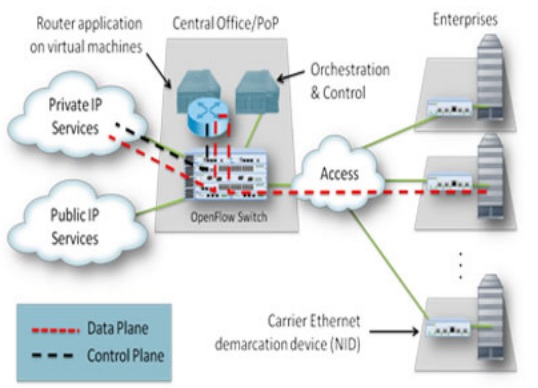
\includegraphics[width=0.9\linewidth]{figure12}}%
%  \subcaptionbox{Another sub-figure\label{fig:rightsubfig}}%
%    {
\includegraphics[width=0.5\linewidth]{knitting-vectorial}}%
  \caption{Network Function Virtualization (NFV)}
  \label{fig:nfv}
\end{figure}

\subsection{OpenFlow}
\label{sec:OpenFlow}

Es un protocolo utilizado para suministrar una interfaz abierta para controlar la conectividad y los flujos de dicha conectividad dentro de una red SDN \textbf{"en inglés Software Defined Networking, SDN"}, es un protocolo extensible por lo que permite a los programadores definir elementos adicionales que permitan al protocolo adaptarse a diferentes redes y a nuevas tecnologías. 
\\
\\
%https://www.opennetworking.org/technical-communities/areas/specification/open-datapath/
Openflow funciona principalmente a través de programas Datapath en donde se define el comportamiento esperado para cada tipo de paquete y el camino que debe tomar dentro de la red, para esto \texttt{esto$\{$OpenFlow$\}$} \footnote{https://www.opennetworking.org/technical-communities/areas/specification/open-datapath/} de \textbf{OFN SDN evolution ver 1.0, Open Networking Foundation, 2016.} utiliza diversos componentes durante su ejecución puede \textbf{Ver figura 4.3 OpenFlow}.
\\
\\
\begin{figure}[htbp]
 \ref{fig:OpenFlow} \textbf{Tomado de:} \textit{sdxcentral.com OpenFlow}.
  \centering
  %\subcaptionbox{\la|bel{fig:leftsubfig}}%
    {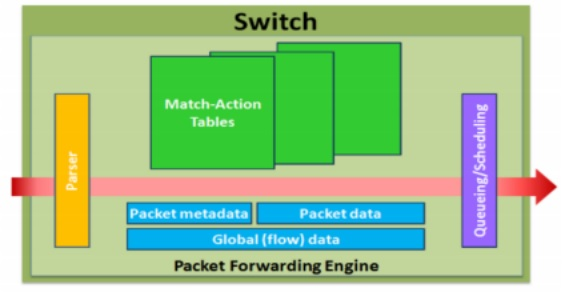
\includegraphics[width=0.7\linewidth]{figure13}}%
%  \subcaptionbox{Another sub-figure\label{fig:rightsubfig}}%
%    {
\includegraphics[width=0.5\linewidth]{knitting-vectorial}}%
  \caption{OpenFlow}
  \label{fig:OpenFlow}
\end{figure}
Cada uno de estos programas de datapath \textbf{Ver figura 4.4 Datapath OpenFlow} es posteriormente compilado para ser ejecutado en el código nativo de cada uno de los vendedores de los dispositivos de hardware, de esta manera el programa de datapath puede ser utilizado independientemente del vendedor del hardware.
\begin{figure}[htbp]
 \ref{fig:DataPath} \textbf{Tomado de:} \textit{sdxcentral.com DataPath OpenFlow}.
  \centering
  %\subcaptionbox{\label{fig:leftsubfig}}%
    {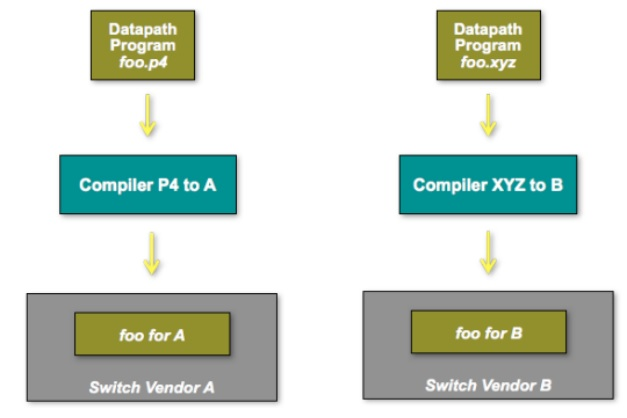
\includegraphics[width=0.7\linewidth]{figure14}}%
%  \subcaptionbox{Another sub-figure\label{fig:rightsubfig}}%
%    {
\includegraphics[width=0.5\linewidth]{knitting-vectorial}}%
  \caption{DataPath OpenFlow}
  \label{fig:DataPath}
\end{figure}

\subsection{NETCONF}
%\label{sec:NETCONF}

\textit{El protocolo se encuentra definido por el estándar \texttt{$\{$RFC6241$\}$} 
\footnote{https://tools.ietf.org/html/rfc6241} \textbf{de la}  IETF \textbf{"Internet Engineering Task Force"} y suministra mecanismos para instalar, manipular y eliminar configuración en dispositivos de red utilizando el formato XML \textbf{ (Lenguaje de Marcado Extensible)}.
\\
\\
NETCONF define un mecanismo simple mediante el cual un dispositivo obtiene una API \textbf{(del inglés API: Application Programming Interface)}, esto con el objetivo de que las aplicaciones utilicen dicha API \textbf{(del inglés API: Application Programming Interface)} para enviar y recibir configuraciones desde y hacia los dispositivos de red, esto utilizando el paradigma RPC \textbf{Remote Procedure Call - Llamada a Procedimiento Remoto} de forma que el cliente codifique en formato XML \textbf{(Lenguaje de Marcado Extensible)} y lo envíe a un servidor, quien responderá con otro XML \textbf{ (Lenguaje de Marcado Extensible)} codificado.}
\\
\\
Conceptualmente el protocolo NETCONF se divide en 4 capas \textbf{Ver figura 4.5 Capas NETCONF}
\begin{figure}[htbp]
 \ref{fig:netconf} \textbf{Tomado de:} \textit{sdxcentral.com NETCONF}.
  \centering
    {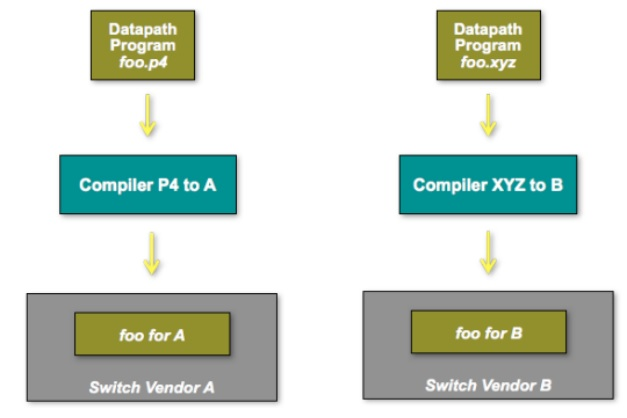
\includegraphics[width=0.7\linewidth]{figure14}}
  \caption{Capas del Protocolo NETCONF}
  \label{fig:netconf}
\end{figure}

\begin{itemize}
\item\textbf{Capa de transporte seguro suministra un camino de comunicación entre cliente y servidor, en general NETCONF puede ser utilizado sobre cualquier protocolo de transporte que cumpla con ciertas características.
}
\item\textbf{La capa de mensajes provee un mecanismo de entramado independiente del transporte para la codificación de RPC \textbf{Remote Procedure Call - Llamada a Procedimiento Remoto} y notificaciones.}
\item\textbf{La capa de operaciones define un set de funciones básicas de protocolos invocados como métodos RPC con parámetros en codificación XML. \textbf{(Lenguaje de Marcado Extensible)}}
\end{itemize}


\subsection{Modelos de datos}
\label{sec:Modelos de datos}

\subsubsection{YANG}
\label{sec:YANG}


Es un lenguaje de modelado de datos que se utiliza para realizar operaciones de datos es estado y configuración del protocolo NETCONF y se encuentra definido bajo el \texttt{$\{$RFC 6020$\}$} 
\footnote{https://tools.ietf.org/html/rfc6020} \textbf{de la} IETF \textbf{"Internet Engineering Task Force"}, YANG modela en forma jerárquica los datos como un árbol y provee una descripción clara de cada nodo así como su relación con otros nodos. YANG define cuatro tipos de nodo para el modelado de datos:

\begin{itemize}
\item[•] \textbf{Nodo Leaf:} contiene datos simples como enteros o cadenas.
\item[•] \textbf{Nodo Leaf-List:}  es una secuencia de nodos "Leaf", en donde cada uno tiene su valor particular.
\item[•]\textbf{Nodo contenedor:} es utilizado para agrupar nodos relacionados en un sub-árbol, este tipo de nodos no tiene valor y sólo tiene nodos hijos. Un contenedor puede contener nodos de cualquier tipo, incluyendo "leaf", "list", "leaf-list" o incluso otros contenedores.
\item[•] \textbf{Nodo Lista:} define una secuencia de entradas de lista identificados por el valor de su "leaf key” una lista puede contener varias de estas llaves y contener cualquier número de nodos de cualquier tipo.
\end{itemize}
YANG permite la definición de RPC de NETCONF, los nombres y parámetros de entrada y salida de las operaciones se encuentran modelados utilizando YANG así como las notificaciones. El siguiente ejemplo muestra como se encuentra estructurado un RPC \textbf{(en inglés, Remote Procedure Call)} en YANG \textbf{ver Script 5.1. Formato JSON \textbf{(JavaScript Object Notation)}}.

\lstset{language=java, caption=RPC Estructura en YANG, label=lst:YANG}
\begin{lstlisting}
/** 
 * JSON es un formato de texto sencillo para el intercambio de datos.  
 */
rpc activate-software-image {
        input {
            leaf image-name {
                type string;
            }
        }
        output {
            leaf status {
                type string;
            }
        }
    }
\end{lstlisting}
En el caso de las interfaces, existe un estándar bajo el \texttt{$\{$RFC 7223$\}$} 
\footnote{https://tools.ietf.org/html/rfc7223} \textbf{de la} IETF \textbf{"Internet Engineering Task Force"} en el que se define una estructura común en YANG para las interfaces de red, como tal la IETF definió la siguiente estructura de datos \textbf{ver Script 5.1. Interfaces:}

\lstset{language=java, caption=Interface YANG, label=lst:Interface}
\begin{lstlisting}
/** 
 * Interfaces
 */
+--rw interfaces
     |  +--rw interface* [name]
     |     +--rw name                        string
     |     +--rw description?                string
     |     +--rw type                        identityref
     |     +--rw enabled?                    boolean
     |     +--rw link-up-down-trap-enable?   enumeration
     +--ro interfaces-state
        +--ro interface* [name]
           +--ro name               string
           +--ro type               identityref
           +--ro admin-status       enumeration
           +--ro oper-status        enumeration
           +--ro last-change?       yang:date-and-time
           +--ro if-index           int32
           +--ro phys-address?      yang:phys-address
           +--ro higher-layer-if*   interface-state-ref
           +--ro lower-layer-if*    interface-state-ref
           +--ro speed?             yang:gauge64
           +--ro statistics
              +--ro discontinuity-time    yang:date-and-time
              +--ro in-octets?            yang:counter64
              +--ro in-unicast-pkts?      yang:counter64
              +--ro in-broadcast-pkts?    yang:counter64
              +--ro in-multicast-pkts?    yang:counter64
              +--ro in-discards?          yang:counter32
              +--ro in-errors?            yang:counter32
              +--ro in-unknown-protos?    yang:counter32
              +--ro out-octets?           yang:counter64
              +--ro out-unicast-pkts?     yang:counter64
              +--ro out-broadcast-pkts?   yang:counter64
              +--ro out-multicast-pkts?   yang:counter64
              +--ro out-discards?         yang:counter32
              +--ro out-errors?           yang:counter32
\end{lstlisting}


\subsection{RESTful APIs}
\label{sec:RESTful APIs}

Una API RESTful, también conocida como servicio web RESTful, se basa en la tecnología de transferencia de estado representacional (REST), un estilo arquitectónico y un enfoque de las comunicaciones a menudo utilizadas en el desarrollo de servicios web.\\
\\
REST utilizado por los navegadores puede considerarse como el idioma de Internet. Con el uso de la nube en aumento, las API \textbf{(del inglés API: Application Programming Interface)} están emergiendo para exponer los servicios web. REST \textbf{(en inglés "representational state transfer")}es una opción lógica para crear API \textbf{(del inglés API: Application Programming Interface)} que permiten a los usuarios conectarse e interactuar con servicios en la nube. Las API RESTful son utilizadas por sitios como Amazon, Google, LinkedIn y Twitter \textbf{Ver figura 4.6 Rest Web Services}.

\begin{figure}[htbp]
 \ref{fig:restfulapi} \textbf{Tomado de:} \textit{restfulapi.net}.
  \centering
  %\subcaptionbox{\label{fig:leftsubfig}}%
    {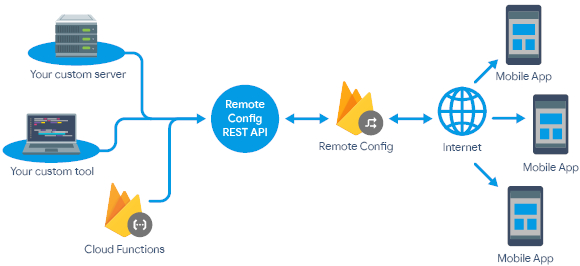
\includegraphics[width=0.8\linewidth]{figure15}}%
%  \subcaptionbox{Another sub-figure\label{fig:rightsubfig}}%
%    {
\includegraphics[width=0.5\linewidth]{knitting-vectorial}}%
  \caption{RestFull API}
  \label{fig:restfulapi}
\end{figure}

\subsection{RESTCONF}
%\label{sec:RESTCONF}

Restconf es un protocolo basado en HTTP \textbf{(en inglés: Hypertext Transfer Protocol o HTTP)} que suministra una interfaz programática para acceder a datos definidos en YANG utilizando los conceptos de datastore definidos en el protocolo NETCONF.
\\
\\
NETCONF y RESTCONF suelen trabajar en conjunto permitiendo la ejecución de operaciones CRUD \textbf{(del original en inglés: Create, Read, Update and Delete)} \textbf{Ver figura 4.7 Estructura RESTCONF}.
\begin{figure}[htbp]
\ref{fig:restfulapi2} \textbf{Tomado de:} \textit{restfulapi.net}.
  \centering
  %\subcaptionbox{\label{fig:leftsubfig}}%
    {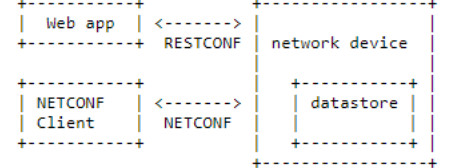
\includegraphics[width=0.6\linewidth]{figure16}}%
%  \subcaptionbox{Another sub-figure\label{fig:rightsubfig}}%
%    {
\includegraphics[width=0.5\linewidth]{knitting-vectorial}}%
  \caption{Estructura RESTCONF}
  \label{fig:restfulapi2}
\end{figure}
Al estar basado en HTTP  \textbf{(en inglés: Hypertext Transfer Protocol o HTTP)} las operaciones CRUD de RESTCONF se realizan mediante los métodos tradicionales, como los son los siguientes:
\begin{itemize}
\item\textbf{Get:} "read or retrieve data"	.
\item\textbf{Post:} "add new data".
\item\textbf{Put:} "update data that already exists".
\item\textbf{Delete:} "remove data".
\end{itemize}

RESTCONF requiere de HTTP \textbf{(en inglés: Hypertext Transfer Protocol o HTTP)} para su transporte y requiere soporte de TLS \textbf{(Transport Layer Security, seguridad de la capa de transporte)} para su transporte, aunque no se especifica que versión, para RESTCONF si se recomienda por lo menos HTTP1.1, dado que los servidores RESTCONF deben soportar HTTPS \textbf{(en inglés: Hypertext Transfer Protocol Secure o HTTPS)}, dichos servidores tienen que presentar un certificado dígital X509v3.

\section{Marco de Referencia Tecnológico}
\label{sec:Marco de referencia tecnológico}

La solución definida en este proyecto es una red IWAN de Cisco, en el capitulo “selección de la solución” en este mismo documento se plantean las razones por las cuales se escogió IWAN \textbf{WAN inteligente de Cisco®} como la mejor solución para el caso de este cliente. Por tanto este apartado estará dedicado a las tecnologías que componen la solución.


\subsection{IWAN}
\label{sec:IWAN}

IWAN \textbf{WAN inteligente de Cisco®} es una solución SD-WAN \textbf{(“Software Defined Networking in Wide Area Networks”)} propietaria de Cisco cuyo objetivo es la reducción de costos para el transporte de la información del cliente al hacer viable mediante una serie de tecnologías la utilización de enlaces menos costosos como internet, en esta solución el tráfico se enruta de manera dinámica según las condiciones de la aplicación, la solución está diseñada para empresas cuyas sucursales tengan un aumento en su tráfico WAN \textbf{(Wide Area Network en inglés)} por el uso de aplicaciones en la nube, Cisco dice ofrecer las siguientes ventajas con su aplicación de IWAN \textbf{Ver figura 4.8 Ventajas de una IWAN}.:

\begin{figure}[htbp]
  \centering
  %\subcaptionbox{\label{fig:leftsubfig}}%
    {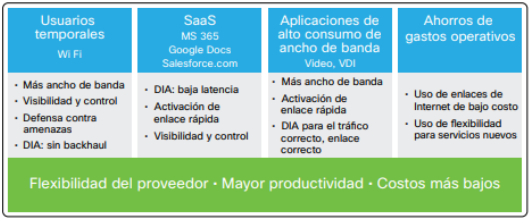
\includegraphics[width=0.7\linewidth]{figure17}}%
%  \subcaptionbox{Another sub-figure\label{fig:rightsubfig}}%
%    {
\includegraphics[width=0.5\linewidth]{knitting-vectorial}}%
  \caption{Ventajas de una IWAN}
  \ref{fig:iwan} \textbf{Tomado de:} \textit{autores}.
  \label{fig:iwan}
\end{figure}
IWAN \textbf{WAN inteligente de Cisco®} se compone de varias tecnologías que hacen de la solución una alternativa efectiva para las sucursales que utilizan tanto consumo de aplicaciones centralizadas como aplicaciones en la nube:
\begin{itemize}
\item[•]\textbf{Independencia de transporte:} la solución utiliza DMVPN \textbf{("Dynamic Multipoint VPN")} para la creación de túneles dinámicos entre todas las sedes, estos túneles se encuentran encriptados para garantizar un componente de seguridad sobre el transporte aunque vaya por la red pública, esto permite obtener una topología "full-mesh" de manera automática y al mismo tiempo obtener una configuración independiente del tipo de transporte y del proveedor de servicios que sea contratado.
\item[•]\textbf{Enrutamiento basado en aplicación:} la solución utiliza además de EIGRP \textbf{(Protocolo de Enrutamiento de Puerta de enlace Interior Mejorado en español)} como protocolo de enrutamiento, una solución propietaria de Cisco llamada  \textit{"Performance Routing"}, que permite tomar decisiones de enrutamiento basándose en el estado actual de los enlaces y en las necesidades de calidad de servicio de cada aplicación.
\item[•]\textbf{Gestión centralizada:} mediante la controladora SDN \textbf{(en inglés Software Defined Networking)} APIC-EM \textbf{"Cisco Application Policy Infrastructure Controller"} es posible gestionar los equipos remotos desde un punto centralizado y realizar cambios a una gran cantidad de dispositivos al mismo tiempo, agilizando y automatizando los cambios de red.
\item[•]\textbf{Optimización de recursos WAN:} la solución incluye una tecnología de compresión de tráfico llamada WAAS \textbf{(Wide Area Augmentation System)} que permite ahorrar costos en los enlaces WAN \textbf{(Wide Area Network en inglés)} haciendo más efectivo el uso del ancho de banda.
\end{itemize}

La controladora SDN \textbf{(en inglés Software Defined Networking)} que utiliza esta tecnología se denomina APIC-EM, esta controladora no solamente cumple la función de plano de control sino que también contiene aplicaciones de red embebidas que aprovechan la naturaleza centralizada de la controladora, entre esas aplicaciones se encuentra IWAN \textbf{"Cisco Application Policy Infrastructure Controller"}, que es la solución SD-WAN \textbf{(“Software Defined Networking in Wide Area Networks”)}puntual que se presenta en este documento, la controladora SDN \textbf{(en inglés Software Defined Networking)} sin embargo es el puente entre la aplicación y la red física, esto puede apreciarse con mayor detalle en la siguiente \textbf{Ver figura 4.9 Estructura de APIC-EM}.
\begin{figure}[htbp]
\ref{fig:cisco} \textbf{Tomado de:} \textit{Software Defined Networking in Wide Area Networks www.cisco.com}.
  \centering
  %\subcaptionbox{\label{fig:leftsubfig}}%
    {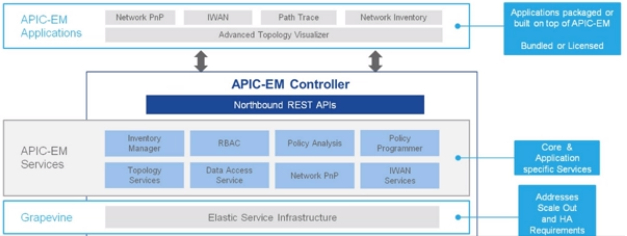
\includegraphics[width=0.8\linewidth]{figure18}}%
%  \subcaptionbox{Another sub-figure\label{fig:rightsubfig}}%
%    {
\includegraphics[width=0.5\linewidth]{knitting-vectorial}}%
  \caption{Estructura de APIC-EM}
  \label{fig:cisco}
\end{figure}

Una de las mayores ventajas de esta controladora es que no necesita de equipos de red especiales que soporten los protocolos de SDN \textbf{(“Software Defined Networking in Wide Area Networks”)}, aunque esto último es lo recomendado el APIC-EM \textbf{"Cisco Application Policy Infrastructure Controller"} trae las ventajas de SDN sin requerir de una gran inversión en cambio de equipos de red, lo que lo hace una opción bastante atractiva para una compañía que quiera empezar a adentrarse en la programabilidad de la red sin requerir una inversión inicial tan fuerte.


\subsection{DMVPN}
%\label{sec:DMVPN}

DMVPN \textbf{(Dynamic Multipoint VPN)} es la solución de transporte propietaria de Cisco que hace parte de la solución de IWAN \textbf{WAN inteligente de Cisco®}, es una solución de \textit{"Overlay"} en donde las ubicaciones remotas establecen un túnel estático hacia una ubicación central(hub) y establece túneles de manera dinámica entre diferentes ubicaciones remotas("spokes").
\\
\\
Esto permite tener conectividad "Full-Mesh" sin tener que realizar las configuraciones de todos los túneles de forma manual, los túneles entre "Spokes" son removidos después de un periodo de inactividad, liberando así recursos de memoria y "CPU" \textbf{(del inglés: central processing unit)} y por tanto eliminando la necesidad de routers tan robustos en las sedes remotas, los equipos de enrutamiento de mayor capacidad deben ser por tanto utilizados en el sitio central (hub). La siguiente \textbf{Ver figura 4.10 DMVPN} muestra el comportamiento dinámico de DMVPN \textbf{(Dynamic Multipoint VPN)}.
\begin{figure}[htbp]
 \textbf{Tomado de:} \textit{www.cisco.com Dynamic Multipoint VPN}.
  \centering
  %\subcaptionbox{\label{fig:leftsubfig}}%
    {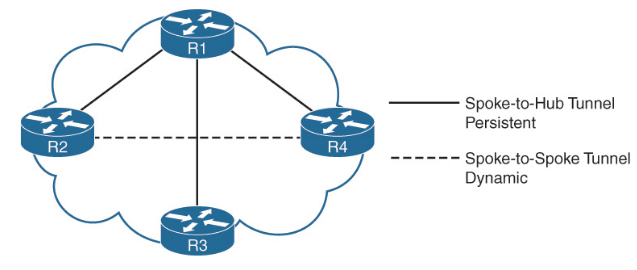
\includegraphics[width=0.9\linewidth]{figure19}}%
%  \subcaptionbox{Another sub-figure\label{fig:rightsubfig}}%
%    {
\includegraphics[width=0.5\linewidth]{knitting-vectorial}}%
  \caption{Dynamic Multipoint VPN}
    \label{fig:dynamic}
\end{figure}

DMVPN \textbf{(Dynamic Multipoint VPN)} utiliza diversas tecnologías para lograr este objetivo, las más relevantes se enuncian a continuación.
\begin{itemize}
\item[•]\textbf{Túneles mGRE:} es un protocolo de entunelamiento capaz de transportar múltiples protocolos como IPv4 \textbf{Internet Protocol version 4}, IPv6 \textbf{Internet Protocol version 6} y otros, estos túneles son asignados a una interface física y requieren direccionamiento propio en la interfaz del túnel, la diferencia entre esta tecnología y los túneles GRE \textbf{(Generic Routing Encapsulation)} tradicionales es que mGRE \textbf{Multipoint Generic Routing Encapsulation} puede conectar más de 2 dispositivos utilizando el mismo túnel \textbf{Ver figura 4.11 Túneles mGRE}.
\begin{figure}[htbp]
\ref{fig:mgre} \textbf{Tomado de:} \textit{www.cisco.com mGRE}.
  \centering
  %\subcaptionbox{\label{fig:leftsubfig}}%
    {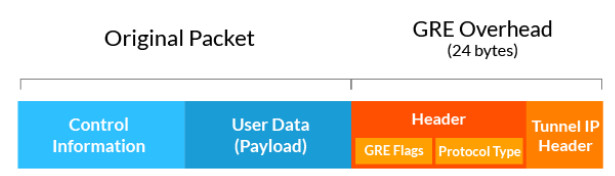
\includegraphics[width=0.7\linewidth]{figure20}}%
%  \subcaptionbox{Another sub-figure\label{fig:rightsubfig}}%
%    {
\includegraphics[width=0.5\linewidth]{knitting-vectorial}}%
  \caption{Túneles mGRE}
  \label{fig:mgre}
\end{figure}
\item[•]\textbf{NHRP:} este protocolo se encuentra definido bajo el \texttt{$\{$RFC 2332$\}$} 
\footnote{https://tools.ietf.org/html/rfc2332}, y es utilizado para que un equipo fuente determine el siguiente salto hacia un destino en una red NBMA \textbf{("non-broadcast multiple access")}, es decir realiza una resolución de direccionamiento, similar a lo que ocurre con ARP \textbf{el inglés Address Resolution Protocol} en la resolución de dirección IP \textbf{(Internet Protocol)} a direccion MAC \textbf{del inglés Medium Access Control}. El protocolo funciona utilizando un NHS  que se encarga de la resolución de direccionamiento dentro de la nube de NHRP, por su parte los equipos NHC \textbf{"New Horizon Communications"} son aquellos que realizan las peticiones de NHRP \textbf{"Next Hop Resolution Protocol"} hacia el NHS. La siguiente \textbf{Ver figura 4.12 Protocolo NHRP:} representa el funcionamiento de NHRP en terminos generales:

\begin{figure}[htbp]
 \textbf{Tomado de:} \textit{www.cisco.com Protocol NHRP}.
  \centering
  %\subcaptionbox{\label{fig:leftsubfig}}%
    {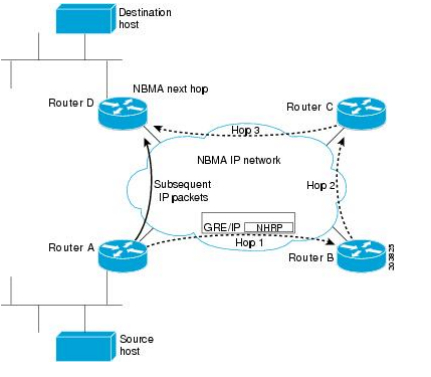
\includegraphics[width=0.8\linewidth]{figure21}}%
%  \subcaptionbox{Another sub-figure\label{fig:rightsubfig}}%
%    {
\includegraphics[width=0.5\linewidth]{knitting-vectorial}}%
  \caption{Protocol NHRP}
  \label{fig:fig2subfig}
\end{figure}
Adicional al registro de los NHC \textbf{"New Horizon Communications"} con los NHS, NHRP \textbf{"Next Hop Resolution Protocol"} tiene la capacidad de que los NHC \textbf{"New Horizon Communications"} encuentren un camino más corto sobre la infraestructura o formar uno mediante una conexión virtual directamente hacia otro NHC \textbf{"New Horizon Communications"}, esta habilidad es utilizada en DMVPN \textbf{ Dynamic Multipoint VPN} para establecer una topología "Full Mesh" sin todo el trabajo administrativo que esto conlleva.
\end{itemize}

\subsection{WAAS}
%\label{sec:WAAS}

Por su parte WAAS \textbf{Wide Area Application Services} es una tecnología propietaria de Cisco que se encarga de optimizar el tráfico TCP \textbf{Transmission Control Protocol} en la red con el principal objetivo de disminuir la utilización de ancho de banda utilizando algoritmos de compresión para este fin. Son varias las tecnologías que reúne WAAS \textbf{Wide Area Application Services} para la optimización del ancho de banda a nivel WAN \textbf{Wide Area Network en inglés}, de ellas vale la pena resaltar las 3 más relevantes.

\begin{itemize}
\item[•]\textbf{TFO Optimization:} utiliza varias tecnologías de optimización de flujo para optimizar el tráfico TCP, realizando funciones como escalamiento de ventanas TCP \textbf{Transmission Control Protocol}, maximización del tamaño de ventana inicial, "Buffering" incrementado, BIC TCP \textbf{Transmission Control Protocol}.
\item[•]\textbf{Compresión:} utiliza algoritmos de eliminación de datos redundantes (DRE) y compresión LZ para optimizar el tráfico WAN \textbf{Wide Area Network en inglés}.
\item[•]\textbf{Aceleración Específica de Aplicaciones:} analiza y predice el tráfico de una aplicación para transformar una secuencia de comandos en una más pequeña, generando así ahorro en la utilización del ancho de banda (BW).
\end{itemize}


\subsection{EIGRP}
\label{sec:EIGRP}

EIGRP \textbf{(Protocolo de Enrutamiento de Puerta de enlace Interior Mejorado en español)} es el protocolo seleccionado por Cisco para hacerse cargo del plano de enrutamiento en la solución \textbf{SD-WAN}, este protocolo aunque Cisco lo considera como un protocolo híbrido con características de protocolos vector distancia y de protocolos estado de enlace, es realmente un protocolo vector distancia ya que no mantiene la topología general del sistema autónomo. Sin embargo este ha demostrado ser un protocolo escalable y de convergencia rápida por lo que se integra adecuadamente en el diseño de IWAN \textbf{WAN inteligente de Cisco®} .
\\
\\
EIGRP \textbf{(Protocolo de Enrutamiento de Puerta de enlace Interior Mejorado en español)} logra una convergencia rápida mediante la construcción de una tabla topológica utilizando la información enseñada por sus vecinos, la diferencia entre esta tabla topológica y la construida por un protocolo de estado de enlace es que  EIGRP \textbf{(Protocolo de Enrutamiento de Puerta de enlace Interior Mejorado en español)} al ser un protocolo vector distancia solo le enseña a sus vecinos las mejores rutas y no todas las rutas que conoce como sería el caso en un protocolo estado de enlace. 
\\
\\
Aún así la convergencia es extremadamente rápida ya que basado en su métrica el protocolo selecciona la mejor ruta (succesor) y la segunda mejor ruta \textit{("Feasable Succesor")}, de esta forma cuando una red deja de aprenderse por la mejor ruta el protocolo utiliza inmediatamente la segunda mejor ruta, por tanto obteniendo unos tiempos de milisegundos para la convergencia.
\\
\\
Para distribuir las rutas a través de la red EIGRP \textbf{(Protocolo de Enrutamiento de Puerta de enlace Interior Mejorado en español)} utiliza actualizaciones de enrutamiento incrementales y no periódicas, esto quiere decir que solo se envía un update cada vez que hay un cambio en la red. EIGRP \textbf{(Protocolo de Enrutamiento de Puerta de enlace Interior Mejorado en español)} depende por lo tanto de sus relaciones de vecinos para propagar de manera confiable los cambios en la tabla de enrutamiento a través de la red. Esta relación de vecindad se forma cuando dos routers corriendo EIGRP \textbf{(Protocolo de Enrutamiento de Puerta de enlace Interior Mejorado en español)} ven los paquetes del otro equipo, estos paquetes son enviados cada 5 segundos.
EIGRP \textbf{(Protocolo de Enrutamiento de Puerta de enlace Interior Mejorado en español)}utiliza una métrica compuesta por los siguientes parámetros para calcular la ruta más corta:

\begin{itemize}
\item\textbf{Ancho de banda:} el menor ancho de banda de la ruta hacia el destino, sin embargo el número utilizado para el cálculo de la métrica.
\item\textbf{Delay:} el retardo total reportado por la interface, sin embargo este valor también es modificado para el calculo de la métrica.
\item\textbf{Load:}el porcentaje de carga(utilización) que tiene el enlace.
\item\textbf{Reliability:} valor configurable administrativamente
\end{itemize}


\subsection{PFR}
\label{sec:PFR}

PFR es parte integral de la solución de IWAN \textbf{WAN inteligente de Cisco®}, y es la mayor responsable de la inteligencia de la solución, su objetivo es mejorar el rendimiento y disponibilidad de las aplicaciones realizando una optimización del control de enrutamiento basándose en los requerimientos de cada aplicación. 
\\
\\
\textbf{PfR} monitorea el rendimiento de red y selecciona el mejor camino basándose en criterios de alcanzabilidad, \textit{"delay", "jitter"} y pérdida de paquetes mientras balancea el tráfico entre los enlaces disponibles.
\textbf{PfR} define varios roles para los dispositivos que componen la solución, dichos roles son \textit{"Master Controler (MC)" y "Border Router (BR)"}, el \textbf{MC} actúa como plano de control para el \textbf{PfR} y el \textbf{BR} sería el plano de datos al seleccionar el camino basándose en las decisiones tomadas por el \textbf{MC}.
\\
\\
En \textbf{PfR} las políticas de tráfico son definidos basados en DSCP o en la aplicación por sí misma, que se identifica mediante "AVC" \textbf{(Application visibility and Control)}. dichas políticas contienen la información de requerimientos en cuanto a parámetros de retardo, \textit{"jitter"} y pérdida de paquetes para cada aplicación así como la preferencia de camino de cada una de ellas. Una vez definida la política \textbf{PfR detecta} el tráfico y comienza a realizar mediciones de ancho de banda y rendimiento, posteriormente el \textbf{MC} toma la decisión mediante la comparación de métricas en tiempo real y le da la instrucción al \textbf{BR} de utilizar el camino apropiado. \textbf{Ver figura 4.13 PfR} muestra el flujo de la operación de \textbf{PfR}:

\begin{figure}[htbp]
 \textbf{Tomado de:} \textit{www.cisco.com SD-WAN Fundamentals and Resources PfR}.
  \centering
  %\subcaptionbox{\label{fig:leftsubfig}}%
    {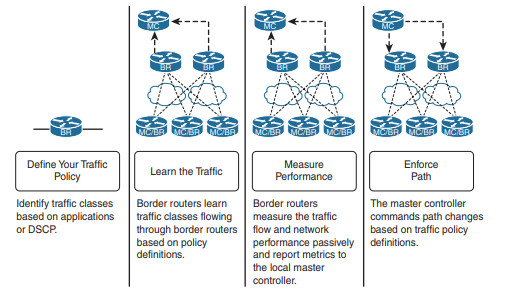
\includegraphics[width=1.1\linewidth]{figure22}}%
%  \subcaptionbox{Another sub-figure\label{fig:rightsubfig}}%
%    {
\includegraphics[width=0.5\linewidth]{knitting-vectorial}}%
  \caption{PfR}
  \label{fig:fig2subfig}
\end{figure}

Dentro de los roles de \textbf{MC y BR} existen dos variantes, los equipos Hub y los \textit{"Branch"}, equipos Hub son los responsables del plano de control en el caso del MC y del plano de datos en el caso del BR para toda la topología de red, el HUB MC se encarga mediante \textbf{SAF} de propagar las políticas, especificaciones de los monitores para medir rendimiento de los canales y prefijos de los sitios a los MC en cada Branch y a los HUB BR, los \textbf{"BRANCH MC"} a su vez propagan las políticas a los \textit{"BRANCH BR"}. La siguiente \textbf{Ver figura 4.14 Branch} detalla este flujo de información entre los elementos de IWAN \textbf{WAN inteligente de Cisco®} . 

\begin{figure}[htbp]
 \textbf{Tomado de:} \textit{www.cisco.com SD-WAN Fundamentals and Resources PfR}.
  \centering
  %\subcaptionbox{\label{fig:leftsubfig}}%
    {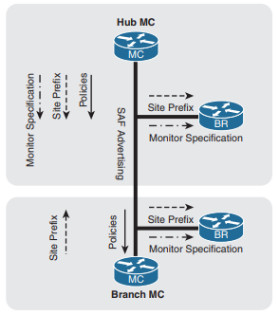
\includegraphics[width=0.5\linewidth]{figure23}}%
%  \subcaptionbox{Another sub-figure\label{fig:rightsubfig}}%
%    {
\includegraphics[width=0.5\linewidth]{knitting-vectorial}}%
  \caption{Branch PFR}
  \label{fig:fig2subfig}
\end{figure}
\section{Open Daylight}
\label{sec:Open Daylight}

El proyecto \textbf{OpenDaylight} es una plataforma de código abierto para \textbf{SDN} que hace
uso de protocolos abiertos para suministrar control centralizado y programático de los
dispositivos de red, así como monitoreo de estos. La plataforma se basa en una arquitectura de "Microservicios" en la que cada microservicio es un protocolo o servicio particular requerido por el usuario durante la instalación de la controladora. La controladora soporta un amplio rango de protocolos de red para su funcionamiento como lo son: \textbf{Openflow, p4 BGP, PCEP, LISP, Netconf, Ovsdb y Snmp}. La capa de abstracción
del servicio se encuentra basada en YANG, el cual se utiliza para crear esquemas de bancos de datos, generar REST API (RESTCONF) y generación automática de código.
\\
\\
OpenDaylight suministra un gran conjunto de servicios de red para diferentes servicios, uno de los más interesantes para este proyecto es el servicio de \textbf{NRO ("Network Resource Optimization")}, en donde los algoritmos en la controladora explotan el hecho de la naturaleza centralizada de una \textbf{SD-WAN}, sus analíticas y su mecanismo de políticas para lograr implementar ingenierıíade tráfico a través de una infraestructura heterogénea. La controladora divide la operación de la red en 4 planos diferentes:
\begin{itemize}
\item[•]\textbf{Elementos del plano de datos:} son los dispositivos físicos que se encargan de dar conectividad a la red, esta es la red tradicional que se conoce normalmente, la diferencia es que los equipos deben soportar Openflow u otro protocolo a través del cual la controladora pueda configurar los equipos.

\item[•]\textbf{Interfaces Southbound:} es la forma de comunicación de la controladora con el resto de la red, esto a través de tecnologías como Openflow o NETCONF.
\item[•]\textbf{Controladora:} consta de la capa de abstracción de servicio \textbf{SAL}, que se encarga
de la abstracción del plano de control de la red de los dispositivos físicos a la controladora y de las funciones de servicios de red, que vienen a ser aplicaciones predefinidas que vienen por defecto sobre la controladora.
\item[•]\textbf{Aplicaciones de Red Orquestación y Servicios:} esta es la capa de la controladora que se encarga de a través de \textbf{RESTful API} permitir la programabilidad de la red y por tanto la automatización de procesos sobre la red. Las funciones de cada una de las capas y la relación entre ellas pueden verse de forma más clara en la siguiente \textbf{Ver figura 4.15 Red Orquestación}

\end{itemize}

\begin{figure}[htbp]
 \textbf{Tomado de:} \textit{opendaylight.org Open Daylight}.
  \centering
  %\subcaptionbox{\label{fig:leftsubfig}}%
    {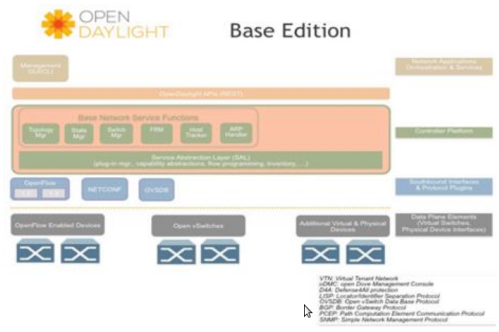
\includegraphics[width=0.9\linewidth]{figure24}}%
%  \subcaptionbox{Another sub-figure\label{fig:rightsubfig}}%
%    {
\includegraphics[width=0.5\linewidth]{knitting-vectorial}}%
  \caption{Red Orquestación Open Daylight}
  \label{fig:fig2subfig}
\end{figure}

Uno de los aspectos clave de la controladora OpenDaylight es MD-SAL("Model Driven Service Abstraction Layer"), el cual autogenera APIs RESTCONF para los objetos en
los modelos de los que aprende, la solución se basa por tanto en RESTCONF y MD-SAL en conjunción con modelos YANG de datos para la configuración de red, colección de estadísticas y orquestación de servicios.\textbf{Ver figura 4.16 Flujo que ocurre entre estos elementos dentro del funcionamiento de la controladora.} muestra el flujo que ocurre entre estos elementos dentro del funcionamiento de la controladora.

\begin{figure}[htbp]
 \textbf{Tomado de:} \textit{opendaylight.org Open Daylight}.
  \centering
  %\subcaptionbox{\label{fig:leftsubfig}}%
    {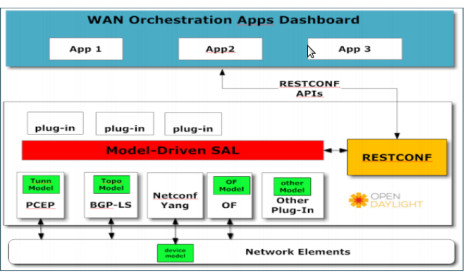
\includegraphics[width=0.9\linewidth]{figure25}}%
%  \subcaptionbox{Another sub-figure\label{fig:rightsubfig}}%
%    {
\includegraphics[width=0.5\linewidth]{knitting-vectorial}}%
  \caption{Funcionamiento de una Controladora}
  \label{fig:fig2subfig}
\end{figure}




\section{Cisco VIPTELA}
\label{sec:Cisco VIPTELA}
La nueva solución SD-WAN de Cisco divide la topología de red en 3 planos diferentes, un plano de datos, uno de control y uno de gestión y orquestación, integrado con su nueva arquitectura DNA, la solución pretende automatizar las configuraciones de red creando una red "Overlay" que permite agilizar las configuraciones y en donde los equipos físicos pasan a un segundo plano en cuanto a gestión de la red, la siguiente
\textbf{Ver figura 4.17 Arquitectura Cisco VIPTELA.}  muestra la arquitectura propuesta por Cisco. 
\\
\\
Es importante notar que los protocolos que corren en el “Underlay” sobre la infraestructura siguen siendo
los mismos que en el caso de IWAN \textbf{WAN inteligente de Cisco®} , es decir PfR, DMVPN y EIGRP \textbf{(Protocolo de Enrutamiento de Puerta de enlace Interior Mejorado en español)} y WAAS como protocolos principales, sin embargo en esta solución lo que cambia es la administración y la gestión, ya que en lugar de la plataforma \textbf{APIC-EM} se tiene un ecosistema más rico en inteligencia de la red, compuesto por el "vManage" como componente principal
encargado de crear nuevos servicios de red en demanda y garantizar la automatización "end-to-end" de toda la infraestructura. Cabe mencionar que IWAN \textbf{WAN inteligente de Cisco®}  sigue siendo una de las aplicaciones más utilizadas dentro del nuevo esquema de \textbf{SD-WAN} de Cisco, la diferencia radica en la controladora y el funcionamiento general de la arquitectura.

\begin{figure}[htbp]
 \textbf{Tomado de:} \textit{www.cisco.com Arquitectura Cisco VIPTELA}.
  \centering
    {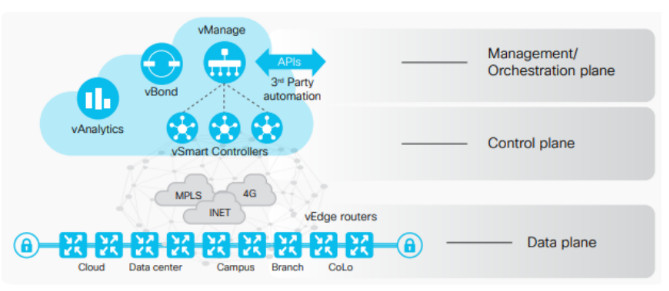
\includegraphics[width=0.9\linewidth]{figure26}}
  \caption{Arquitectura Cisco VIPTELA.}
  \label{fig:fig2subfig}
\end{figure}

\section{NSX SD-WAN}
\label{sec:NSX SD-WAN}


Esta solución de "Vmware" se encuentra desarrollada en base a un "appliance" que actúa como \textbf{CPE} especialmente diseñado para la función de SD-WAN de NSX, aunque también es posible utilizar una \textbf{VNF} de \textbf{CPE} para este propósito. Este dispositivo utiliza \textbf{"Dynamic Multipath Optimization" (DMO)} y "deep application recognition" agregan múltiples enlaces y dirige el tráfico sobre los enlaces óptimos. La solución se divide en 3 componentes diferentes listados a continuación:
\begin{itemize}
 
\item[•]\textbf{NSX-SDWAN Gateway:} proporciona rutas de datos optimizadas para las aplicaciones, las sucursales y los centros de datos, al mismo tiempo que da la capacidad de brindar servicios de redes en la nube.
\item[•]\textbf{NSX-SDWAN Edge:} ofrecen conectividad a apliaciones, híbridas, privadas y públicas, este componente puede encontrarse en forma de dispositivo físico o en forma de instancia virtual.
\item[•]\textbf{NSX-SDWAN Orchestrator:} es el componente de la solución que contiene la inteligencia y la automatización, su objetivo es habilitar el aprovisionamiento de servicios virtuales de forma ágil y automatizada. La distribución de estos componentes dentro de la solución.
\textbf{Ver figura 4.18 Distribución de los Componentes.}
\end{itemize}

\begin{figure}[htbp]
 \textbf{Tomado de:} \textit{www.cisco.com Arquitectura Cisco VIPTELA}.
  \centering
  %\subcaptionbox{\label{fig:leftsubfig}}%
    {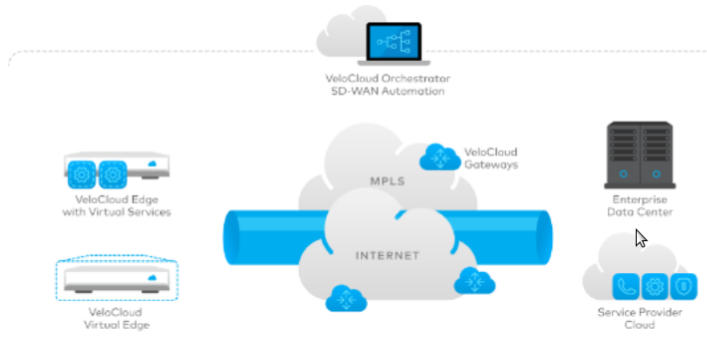
\includegraphics[width=0.8\linewidth]{figure27}}
  \caption{Distribución de los Componentes}
  \label{fig:fig2subfig}
\end{figure}

\section{WAN definida por software (SD-WAN)}
\label{WAN definida por software (SD-WAN)}

La red de área amplia definida por software \textbf{(SD-WAN o SDWAN)} es una aplicación específica de la tecnología de \textbf{red definida por software (SDN)} aplicada a conexiones \textbf{WAN como Internet de banda ancha, 4G, LTE o MPLS}.
Conecta redes empresariales, incluidas sucursales y centros de datos, en grandes distancias geográficas. Se puede usar una WAN, por ejemplo, para conectar sucursales a una red central corporativa o para conectar centros de datos separados por distancia.
\\
En el pasado, las conexiones WAN a menudo usaban tecnología que requería hardware  \textbf{Ver figura 4.19 WAN definida por software (SD-WAN)} propietario especial. SD-WAN, por otro lado, utiliza Internet o una red privada nativa de la nube. SD-WAN desacopla la red del plano de gestión y separa las funciones de gestión y supervisión del tráfico del hardware. 
\begin{figure}[htbp]
 \textbf{Tomado de:} \textit{www.cisco.com SD-WAN}.
  \centering
    {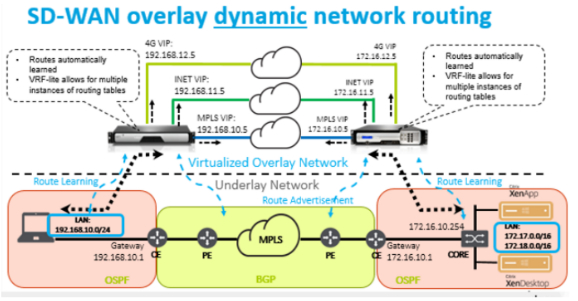
\includegraphics[width=0.7\linewidth]{figure28}}
  \caption{WAN definida por software (SD-WAN)}
  \label{fig:fig2subfig}
\end{figure}

Se basa en cuatro componentes centrales:

\begin{itemize}
\item[•]\textbf{Abstracción de conectividad de borde}
\item[•]\textbf{Virtualización WAN}
\item[•]\textbf{Gestión centralizada y dirigida por políticas}
\item[•]\textbf{Gestión elástica del tráfico}
\end{itemize}